\documentclass[12pt, a4paper]{article}
\usepackage{listings}
\usepackage{paracol}
\usepackage[left=20mm, right=20mm, top=25mm, bottom=25mm]{geometry}
\usepackage{fancyhdr}
\usepackage{xcolor}
\usepackage{graphicx}
\usepackage{float}

\usepackage{titling}
\setlength{\droptitle}{-2cm}

\usepackage{xeCJK}
\setCJKmainfont[AutoFakeBold=true, AutoFakeSlant=true]{DFKai-SB}
\setCJKmonofont[AutoFakeBold=true, AutoFakeSlant=true]{DFKai-SB}
\setCJKsansfont[AutoFakeBold=true, AutoFakeSlant=true]{DFKai-SB}

\usepackage{setspace}
\setstretch{1.1}

\pagestyle{fancy}
\fancyhf{}
\fancyhead[L]{\textbf{Cross Pointer}} % Left header
\fancyhead[C]{\textit{By HyperSoWeak}} % Center header
\fancyhead[R]{\today} % Right header
\fancyfoot[C]{\thepage} % Center footer with page number

\setlength{\headheight}{15pt}

\lstset{
    frame=single, % Use a single frame around the code
    basicstyle=\ttfamily, % Typewriter font for code
    columns=flexible, % Flexible column width
    keepspaces=true, % Keep spaces in code
    breaklines=true, % Allow line breaking
    backgroundcolor=\color{white}, % Background color of the listing
    rulecolor=\color{black}, % Color of the frame
    xleftmargin=10pt, % Left padding
    xrightmargin=10pt, % Right padding
    aboveskip=5pt, % Space above the box
    belowskip=5pt, % Space below the box
    framexleftmargin=5pt, % Left margin inside frame
    framexrightmargin=5pt, % Right margin inside frame
    framexbottommargin=0pt, % Bottom margin inside frame
    framextopmargin=5pt % Top margin inside frame
}


\begin{document}

\begin{center}
    \parbox{0.8\textwidth}{
        \centering
        \vspace{0.5em}
        \LARGE \textbf{Cross Pointer}\\[0.5em]
        \large{Time limit: 1s}\\
        \large{Memory limit: 256MB}\\[0.8em]
    }
\end{center}
\thispagestyle{fancy}

\section*{Problem Description}
你會拿到一個整數指標陣列 \texttt{ptrs},其中每個指標指向另一個整數陣列中的元素。你要實作一個函數 \texttt{count\_cross} 用來計算指標箭頭之間的交叉次數,如下圖所示。

\begin{figure}[H]
    \centering
    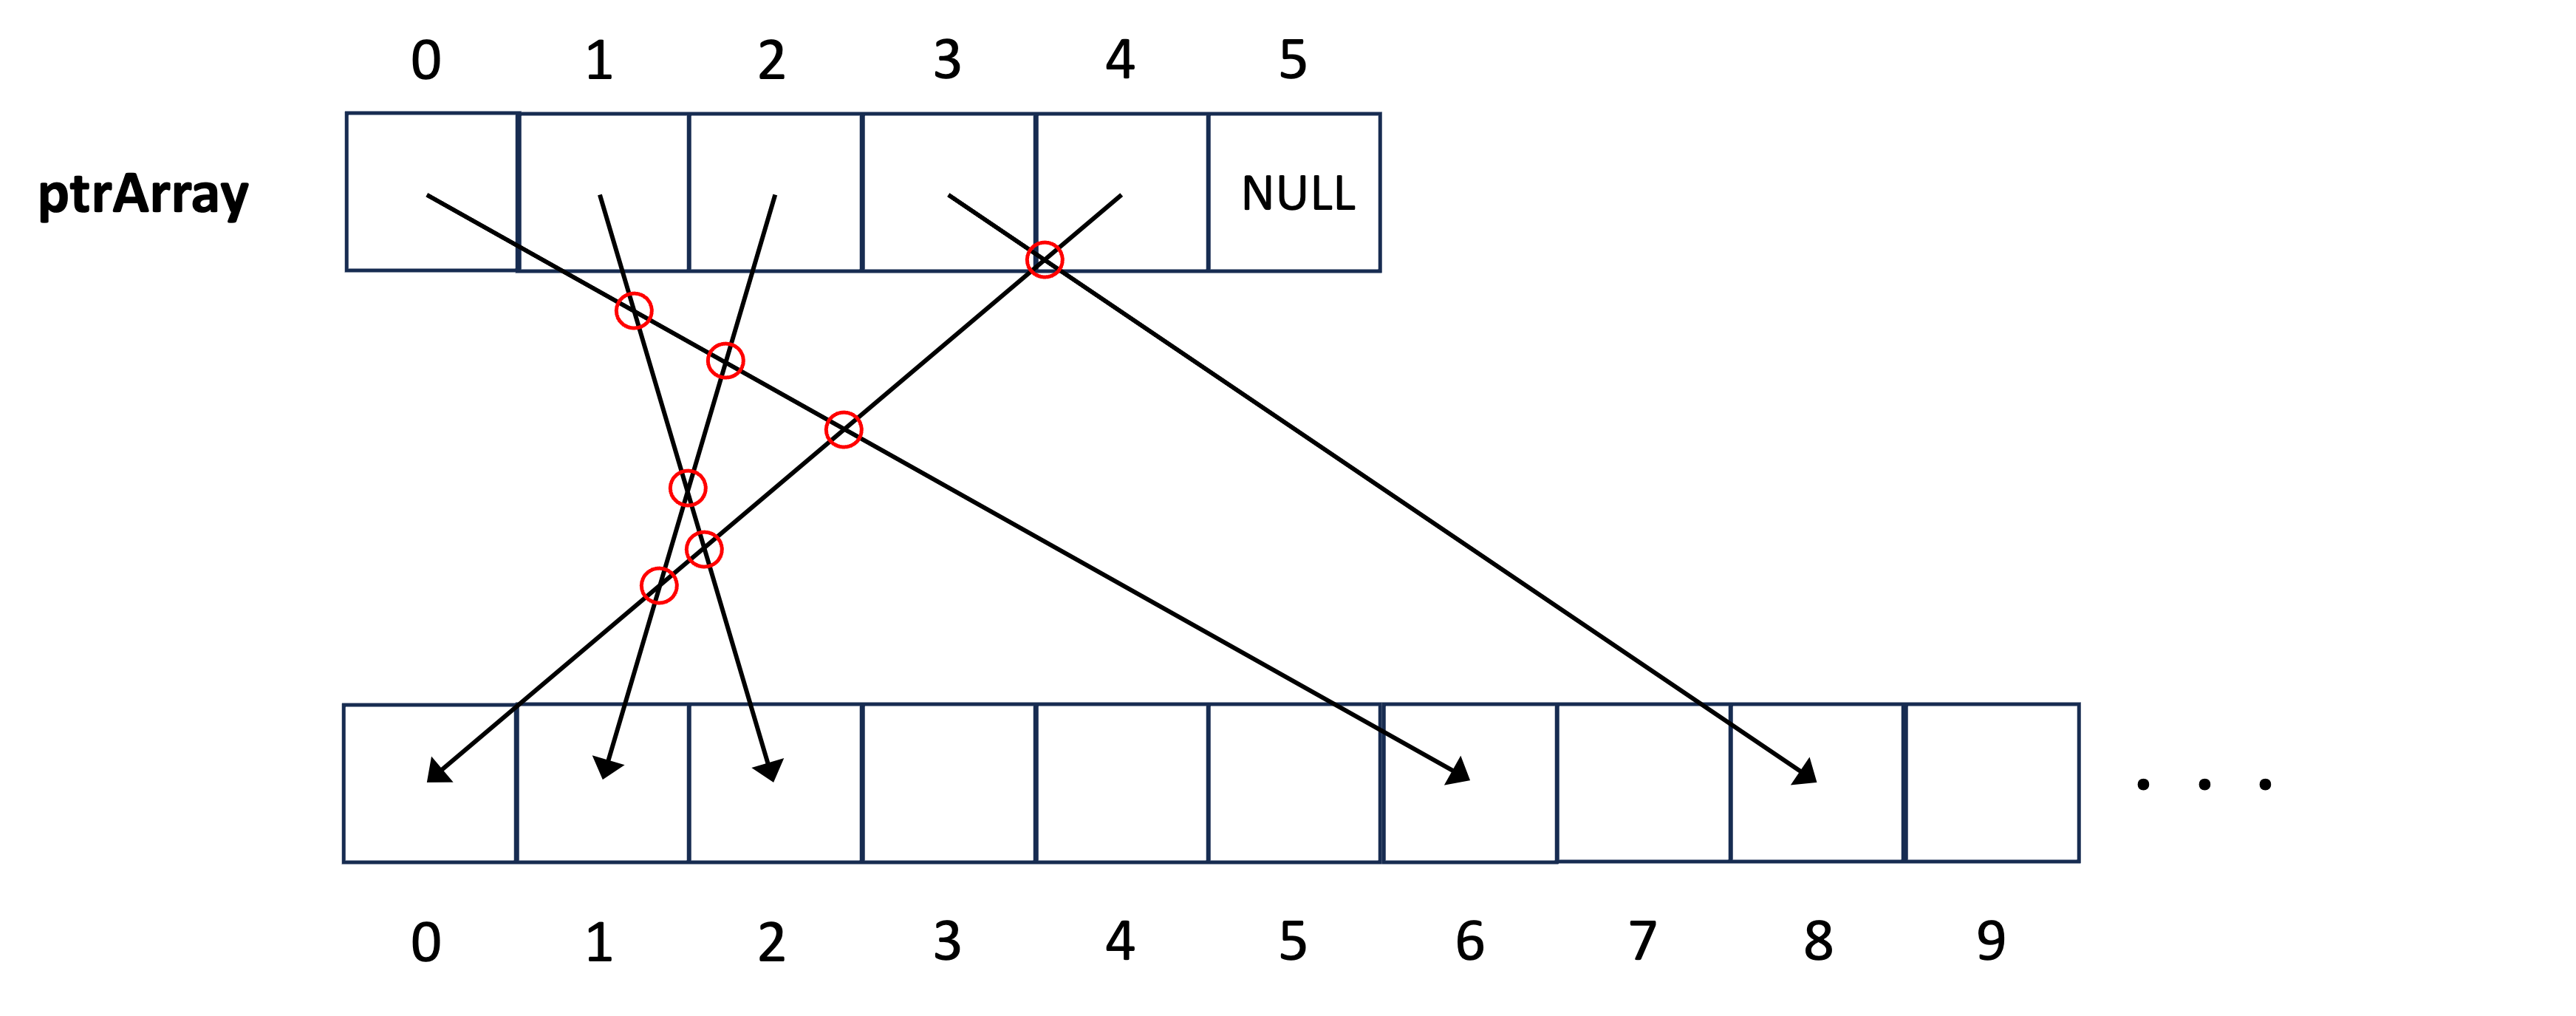
\includegraphics[width=0.8\textwidth]{./pointer.png}
\end{figure}

模板已附在 \texttt{/statement} 中,你只需要實作 \texttt{count\_cross} 函數即可。

\section*{Constraints}
\begin{itemize}
    \item $\texttt{ptrs.size()} \le 1000$
\end{itemize}

\begin{paracol}{2}
    \subsection*{Sample Input 1}
    \begin{lstlisting}
5
6 2 1 8 0
    \end{lstlisting}
    \switchcolumn
    \subsection*{Sample Output 1}
    \begin{lstlisting}
7
    \end{lstlisting}
\end{paracol}

\end{document}
